\documentclass{beamer}
\title{Presentation}
\author{Joseph Siu}
\institute{MCV4U - Ms. Issaeva}
\date{2023/4/11}

\usepackage{amssymb}




\begin{document}

\frame{\titlepage}

%Question Page
\begin{frame}
    \frametitle{Question}
    A snail is traveling along a straight path. The snail's velocity can be modeled by $v(t) = 1.4\ln(1+t^2)$ inches per minutes for $0\leq t\leq 15$ minutes.
    \begin{itemize}
        \item<1-> (a) Find the acceleration of the snail at time $t=5$ minutes.
        \item<2-> (b) What is the displacement of the snail over the interval $0\leq t\leq 15$ minutes?
        \item<3-> (c) At what time t, $0\leq t\leq 15$, is the snail's instantaneous velocity equal to its average velocity over the interval $0\leq t\leq 15$ ?
        \item<4-> (d) An ant arrives at the snail's starting position at time $t=12$ minutes and follows the snail's path. During the interval $12\leq t\leq 15$ minutes, the ant travels in the same direction as the snail with a constant acceleration of 2 inches per minute per minute. The ant catches up to the snail at $t=15$ minutes. The ant's velocity at time $t=12$ is $B$ inches per minute. Find the value of $B$. 
    \end{itemize}
\end{frame}









%Part A
\begin{frame}
    \frametitle{Part A - Find the acceleration of the snail at time $t=5$ minutes.}
    $d(t)$ = displacement \newline
    $v(t) = \frac{dd}{dt} = d'(t)$ = velocity \newline
    $a(t) = \frac{d^2d}{dt^2} = v'(t) = d''(t)$ = acceleration \newline
    \pause
    
    $v(t) = 1.4\ln(1+t^2), t\in [0,15]$ \newline
    $a(t) = v'(t) = \frac{d}{dt}(1.4\ln(1+t^2))$
\end{frame}

\begin{frame}{Part A - Find the acceleration of the snail at time $t=5$ minutes.}
    \begin{align*}
        a(t) &= \frac{d}{dt}(1.4\ln(1+t^2))\\
        &= 1.4\frac{d}{dt}(\ln(1+t^2))\\
        &= 1.4\times \frac{1}{1+t^2} \times \frac{d}{dt}(1+t^2)\\
        &= 1.4\times \frac{1}{1+t^2} \times 2t\\
        &= \frac{2.8t}{1+t^2}\\
    \end{align*}
\end{frame}

\begin{frame}{Part A - Find the acceleration of the snail at time $t=5$ minutes.}
    \begin{align*}
        \left. a(t)\right|_{t=5} &= \left. \frac{2.8t}{1+t^2}\right|_{t=5} \\
        &= \frac{2.8\times 5}{1 + 5^2} = \frac{14}{26} = \frac{7}{13} \\
        &\approx 0.53846153846 (\text{inch per minute per minute})\\
        &\approx 0.538 (\text{inch per minute per minute}) 
    \end{align*}

    Therefore, the acceleration of the snail at time $t=5$ minutes is $\frac{7}{13}$, or approximately 0.538 inch per minute per minute.
\end{frame}

\begin{frame}{Part A - Verify using TI-83 Plus}
    %add images here
    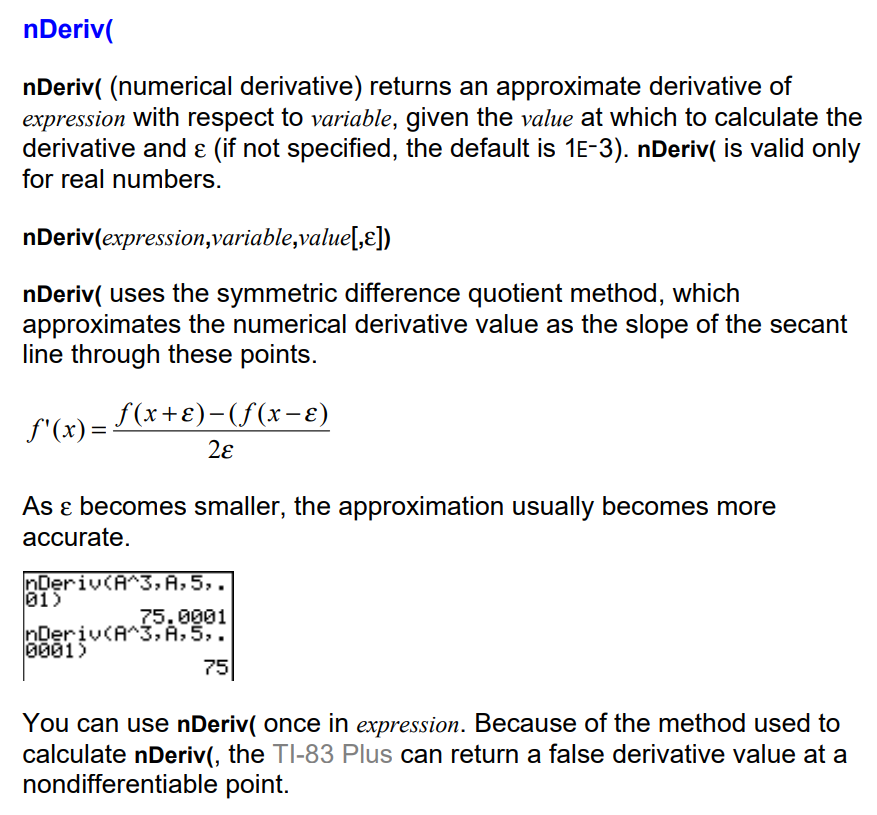
\includegraphics[scale=0.34]{1}
    \tiny \url{https://education.ti.com/en/guidebook/details/en/ABF6D3DD944745A7A76609E97F84B1F7/83p}
\end{frame}

\begin{frame}{Part A - Verify using TI-83 Plus}
    %add images here
    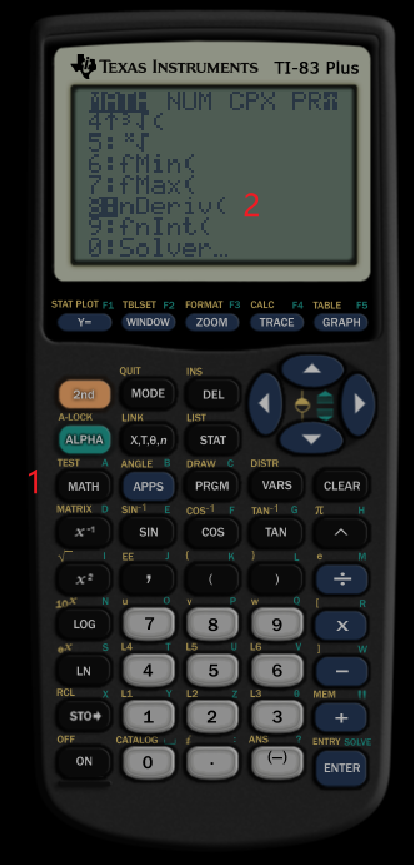
\includegraphics[scale=0.32]{2}
    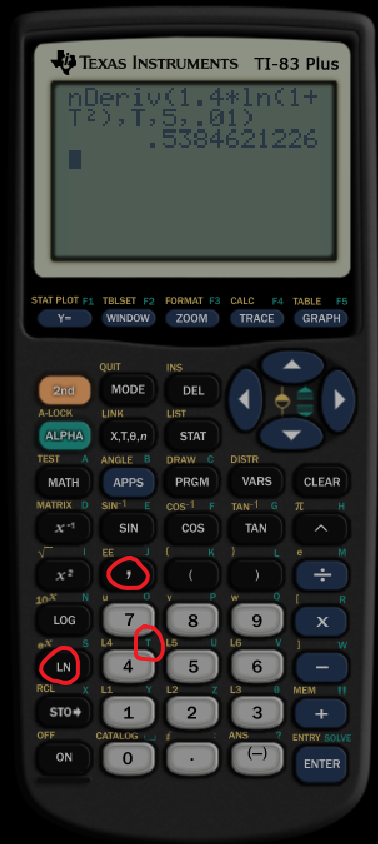
\includegraphics[scale=0.33]{3}
    \tiny \url{https://archive.org/details/ti83p-calculator}
\end{frame}





%Part B
\begin{frame}{Part B - What is the displacement of the snail over the interval $0\leq t\leq 15$ minutes?}
    $d(t)$ = displacement \newline
    $v(t) = \frac{dd}{dt} = d'(t)$ = velocity \newline
    $d(t) = \int d'(t)dt + C = \int v(t)dt + C$ \newline
    \pause
    
    $v(t) = 1.4\ln(1+t^2), t\in [0,15]$ \newline
    $d(t) = \int v(t)dt + C = \int 1.4\ln(1+t^2)dt + C$ \newline \newline
    \begin{align*}
    d(t)_{[0,15]} &= \int_0^{15} 1.4\ln(1+t^2)dt\\
    &= 1.4 \int_0^{15} \ln(1+t^2)dt
    \end{align*}
\end{frame}

\begin{frame}{Part B - What is the displacement of the snail over the interval $0\leq t\leq 15$ minutes?}
    To solve this definite integral, integration by parts is useful.

    Proof can be found at  \hyperlink{https://www.mathcentre.ac.uk/resources/uploaded/mc-ty-parts-2009-1.pdf}{www.mathcentre.ac.uk/resources/uploaded/mc-ty-parts-2009-1.pdf}

    The integration by parts formula states:
    \begin{align*}
    \int_a^b u(x)v'(x)\, dx &= \bigg[u(x)v(x)\bigg]_a^b - \int_a^b u'(x)v(x)\, dx\\
    &= u(b)v(b) - u(a)v(a) - \int_a^b u'(x)v(x)\, dx\\
    \int_a^b u \, dv &= \bigg[uv\bigg]_a^b - \int_a^b v \, du\\
    \end{align*}
\end{frame}

\begin{frame}{Part B - What is the displacement of the snail over the interval $0\leq t\leq 15$ minutes?}
    \begin{align*}
    \int_a^b u \, dv &= \bigg[uv\bigg]_a^b - \int_a^b v \, du\\
    d(t)_{[0,15]} &= 1.4 \int_0^{15} \ln(1+t^2) \, dt\\
    u&=ln(1+t^2)\\
    \frac{du}{dt}=\frac{d}{dt}(ln(1+t^2)) &= \frac{2t}{1+t^2}\\
    du&=\frac{2t}{1+t^2} \, dt\\
    v=t, a&=0, b=15\\
    \int_0^{15} \ln(1+t^2) \, dt &= \bigg[\ln(1+t^2)\times t\bigg]_0^{15} - \int_0^{15} \frac{2t^2}{1+t^2} \, dt\\
    \end{align*}
\end{frame}

\begin{frame}{Part B - What is the displacement of the snail over the interval $0\leq t\leq 15$ minutes?}
    \begin{align*}
    \int_0^{15} \ln(1+t^2) \, dt &= \bigg[\ln(1+t^2)\times t\bigg]_0^{15} - \int_0^{15} \frac{2t^2}{1+t^2} \, dt\\
    &= \bigg[t\ln(1+t^2)\bigg]_0^{15} - 2\int_0^{15} \frac{t^2}{1+t^2} \, dt\\
    &= \bigg[t\ln(1+t^2)\bigg]_0^{15} - 2\int_0^{15} \bigg(1-\frac{1}{1+t^2}\bigg) \, dt\\
    &= \bigg[t\ln(1+t^2)\bigg]_0^{15} - 2\int_0^{15} 1 \, dt + 2\int_o^{15} \frac{1}{1+t^2} \, dt\\
    &= \bigg[t\ln(1+t^2)\bigg]_0^{15} - 2t\bigg|_0^{15} + \left. 2\arctan(t)\right\bigg|_0^{15}\\
    \end{align*}
\end{frame}

\begin{frame}{Part B - What is the displacement of the snail over the interval $0\leq t\leq 15$ minutes?}
    \begin{align*}
    d(t)_{[0,15]} &= 1.4 \int_0^{15} \ln(1+t^2) \, dt\\
    &=1.4\times \bigg(\bigg[t\ln(1+t^2)\bigg]_0^{15} - 2t\bigg|_0^{15} + \left. 2\arctan(t)\right\bigg|_0^{15} \bigg)\\
    &=1.4\times \big[15\ln(1+15^2)-0\ln(1+0^2)-2\times15\\
    &\; -2\times0+2\times\arctan(15)-2\times\arctan(0) \big]\\
    &=1.4\times [15\ln(226)-30+2\arctan(15)]\\
    &\approx 76.04307384 (\text{inches})\\
    &\approx 76.043 (\text{inches})
    \end{align*}
    Therefore, the displacement of the snail over the interval $0\leq t\leq 15$ minutes is $1.4\times [15\ln(226)-30+2\arctan(15)]$, or approximately 76.043 inches (make sure calculator is in radians).
\end{frame}

\begin{frame}{Part B - Verify using TI-83 Plus}
    %add images here
    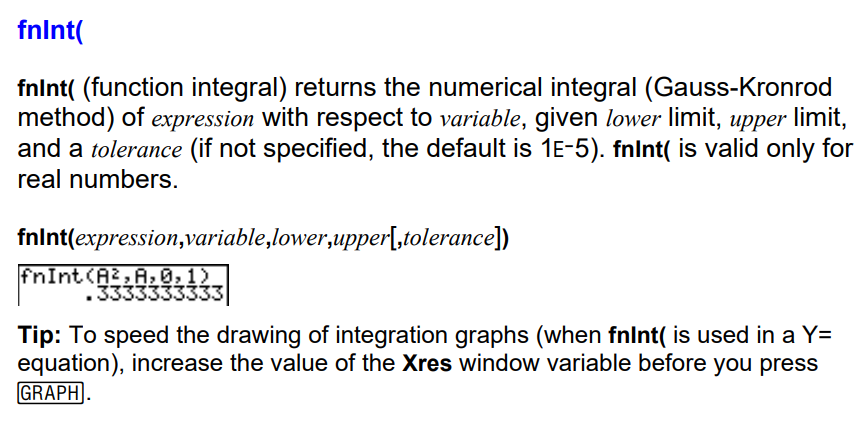
\includegraphics[scale=0.4]{4}
    \tiny \url{https://education.ti.com/en/guidebook/details/en/ABF6D3DD944745A7A76609E97F84B1F7/83p}
\end{frame}

\begin{frame}{Part B - Verify using TI-83 Plus}
    %add images here
    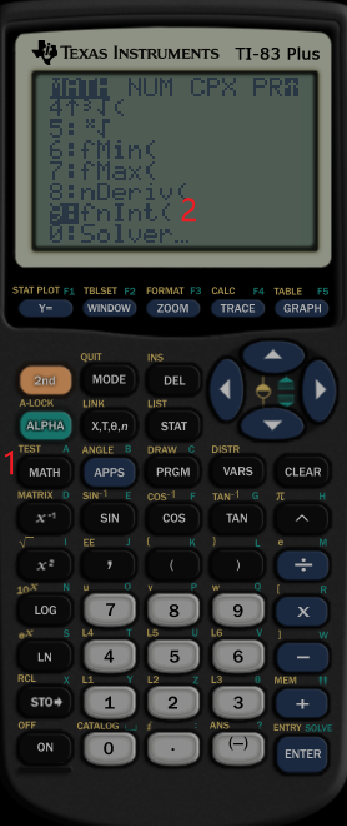
\includegraphics[scale=0.33]{5}
    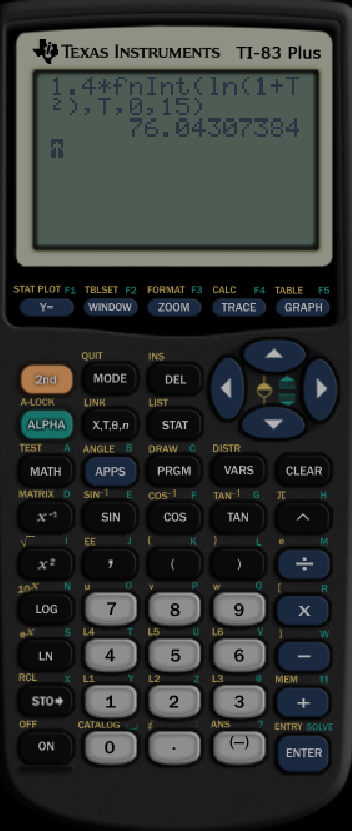
\includegraphics[scale=0.33]{6}
    \tiny \url{https://archive.org/details/ti83p-calculator}
\end{frame}








%Part C
\begin{frame}{Part C - At what time t, $0\leq t\leq 15$, is the snail's instantaneous velocity equal to its average velocity over the interval $0\leq t\leq 15$?}
    \begin{align*}
    v_{ins}&=1.4\ln(1+t^2)\\
    v_{avg}\bigg|_0^{15}&=\frac{d(15)-d(0)}{15-0}\\
    &=\frac{1}{15}d(t)_{[0,15]}\\
    &=\frac{1}{15}\times1.4\times (15\ln(226)-30+2\arctan(15))\\
    &\approx 5.069538256 (\text{inches per minute})\\
    \end{align*}
\end{frame}

\begin{frame}{Part C - At what time t, $0\leq t\leq 15$, is the snail's instantaneous velocity equal to its average velocity over the interval $0\leq t\leq 15$?}
    \begin{align*}
    1.4\ln(1+t^2) &= \frac{1}{15}\times1.4\times (15\ln(226)-30+2\arctan(15))\\
    \ln(1+t^2) &= \frac{1}{15}\times (15\ln(226)-30+2\arctan(15))\\
    t&=\pm \sqrt{e^{\frac{15\ln(226)-30+2\arctan(15)}{15}}-1}\\
    &\approx\pm 6.031468742 (\text{minutes})\\
    \because t &\in [0,15]\\
    \therefore t &= 6.031468742 (\text{minutes})\\
    \therefore t &= 6.031 (\text{minutes})
    \end{align*}
    Therefore, at approximately 6.031 minutes, the snail's instantaneous velocity is equal to its average velocity over the interval $0\leq t\leq 15$.
\end{frame}

\begin{frame}{Part C - Verify using TI-83 Plus}
    %add images here
    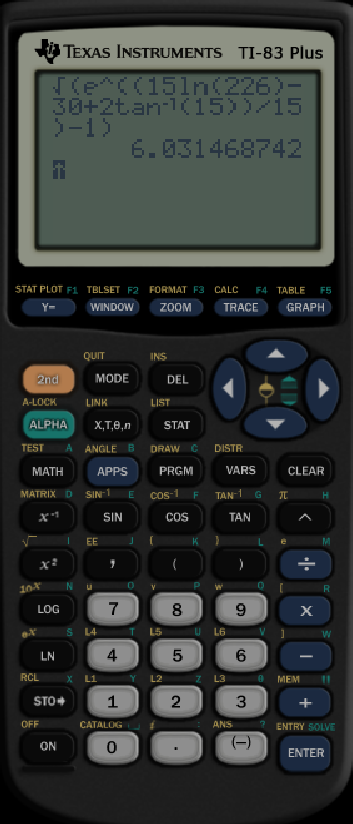
\includegraphics[scale=0.33]{7}\\
    \tiny \url{https://archive.org/details/ti83p-calculator}
\end{frame}













%Part D
\begin{frame}{Part D - [...] Find the value of $B$.}
    \begin{align*}
    a_1(t)&=2\\
    v_1(t)&=\int a_1(t) \, dt + C = \int 2 \, dt + C = 2t + C\\
    \because v_1(12)&=2(12)+C=24+C=B\\
    \therefore B&=C+24\\
    d_1(t)_{[12,15]} &= \int_{12}^{15} v_1(t) \, dt = \int_{12}^{15} (2t+C) \, dt\\
    &= (t^2+Ct)\bigg|_{12}^{15} = 15^2-12^2+15C-12C\\
    &=81+3C
    \end{align*}
\end{frame}

\begin{frame}{Part D - [...] Find the value of $B$.}
    \begin{align*}
    d_1(t)_{[12,15]} &= d(t)_{[0,15]}\\
    81+3C &=1.4\times (15\ln(226)-30+2\arctan(15))\\
    C &= \frac{1.4\times (15\ln(226)-30+2\arctan(15))-81}{3}\\
    B &= 24 + \frac{1.4\times (15\ln(226)-30+2\arctan(15))-81}{3}\\
    &\approx 24-1.65230872 (\text{inches per minute})\\
    &\approx 22.34769128 (\text{inches per minute})\\
    &\approx 22.348 (\text{inches per minute})
    \end{align*}
    Therefore, the velocity of the ant at t=12 minutes is approximately 22.348 inches per minute, the value of B is around 22.348. 
\end{frame}

\begin{frame}{Part D - Verify using TI-83 Plus}
    %add images here
    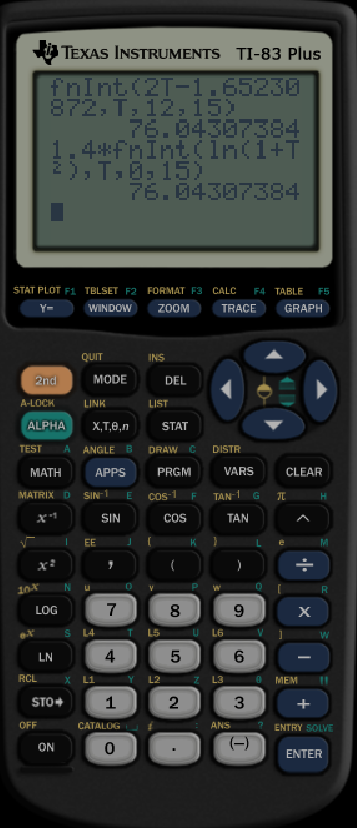
\includegraphics[scale=0.33]{8}\\
    \tiny \url{https://archive.org/details/ti83p-calculator}
\end{frame}








\begin{frame}
    \large Thank You.     
\end{frame}

\end{document}